\chapter{Background Theory}
\label{chapter:background}

\section{Data-driven Algorithm Design}

\todo[inline]{Explanation of best algorithm selection}

This increasing amount of data allows us improve the learning capabilities of machines. We know how well existing algorithms perform for any kind of data and which runtime guarantees they have. However, the algorithms' guarantees are general observations and can vary a lot between different data. In many real-world applications the data does not vary that much, e.g. the data for clustering websites into different types may vary quite much on a yearly base, but as this task gets executed thousands of times each second for certain search algorithms, the data will not change much. By assuming a static context, it is then possible to leverage the context to improve the algorithmic results, e.g. say you want to cluster person data for different genders. By having this a-priori information, you can use a k-means clustering algorithm with $k = 3$ in order to differentiate between female, male and non-binary people.\\

However, such observations are mostly not that trivial and often require more effort in order to obtain useful a-priori information. In order to cluster financial standing, one could imagine seeing different clusters depending on the age or the education. But how many clusters would result here? The data has to be processed and evaluated for different values in this case.\\

Once our algorithm performs well for our data and our tasks, we then want to transfer the gained knowledge to different tasks. Say the algorithm already learned how to differentiate images of the handwritten digits zero, one and two, the same algorithm should then be able to apply the gained knowledge to distinguish between other handwritten digits too. The gained knowledge is some kind of learned data, that can for example be the feature representation of a Convolutional Neural Network, where a potential goal can be to transfer the representation knowledge to another classification task.\\

For clustering tasks learned knowledge could be a number of clusters, a good feature representation for the input data or other useful information that allows performing similar clustering tasks better by transferring the knowledge.

\section{Linkage-based hierarchical clustering.}

This thesis focuses on agglomerative hierarchical clustering, i.e. clustering algorithms that merge clusters starting from each cluster as its own point until all points belong to the same cluster. At each iteration the clusters with the closest distance are merged together. As there are various clustering algorithms, there also are various distance measurements. One way of describe the distance between two clusters, say $X$ and $Y$ is by defining a linkage between them. There are three different methods to do so.

\paragraph{Single Linkage.}

Single linkage defines a distance between two clusters $X$ and $Y$ as the distance between the two nearest points of these clusters (see equation \ref{eq:singlelinkage}).

\begin{equation}
    \begin{aligned}
        d_{SL}(X,Y) = \min\limits_{x \in X, y \in Y} d(x,y)
    \end{aligned}
    \label{eq:singlelinkage}
\end{equation}

\paragraph{Complete Linkage.}

Complete linkage defines a distance between two clusters $X$ and $Y$ as the distance between the two farthest points of these clusters (see equation \ref{eq:completelinkage}).

\begin{equation}
    \begin{aligned}
        d_{CL}(X,Y) = \max\limits_{x \in X, y \in Y} d(x,y)
    \end{aligned}
    \label{eq:completelinkage}
\end{equation}

\paragraph{Average Linkage.}

Average linkage defines a distance between two clusters $X$ and $Y$ as the average distance between all points $x \in X$ and all points $y \in Y$ (see equation \ref{eq:averagelinkage}).

\begin{equation}
    \begin{aligned}
        d_{AL}(X,Y) = \frac{1}{|X||Y|}\sum\limits_{x \in X, y \in Y} d(x,y)
    \end{aligned}
    \label{eq:averagelinkage}
\end{equation}

\paragraph{Effects of different linkage strategies.}

Depending on the linkage strategy, the pairwise distances between all $N$ clusters $C_1, ..., C_N$ will be different. As the clustering algorithm merges the closest pair of clusters in each iteration, the merging clusters $C_i$ and $C_j$ with $i, j \in 1,...,N$ might vary as shown in figure \ref{fig:linkage_effects}, where ten clusters $C_0, ..., C_9$ get clustered with bottom-up hierarchical clustering using the Euclidean distance as distance $d(x,y)$ to calculate the pairwise distance according to the three mentioned linkage strategies.

\begin{figure}[h]
    \centering
    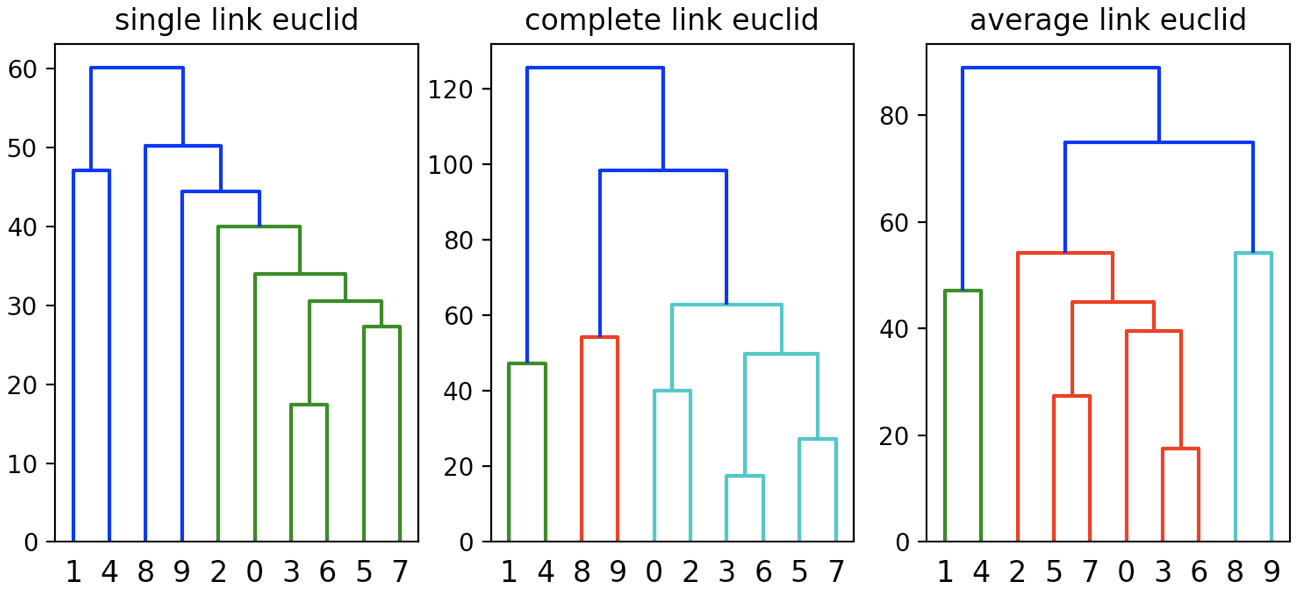
\includegraphics[width=0.8\textwidth]{images/linkage_effects}
    \caption{Different distance measurements often result in different merges for bottom-up hierarchical clustering algorithms. The three discussed linkage strategies result in three different clusterings.}
    \label{fig:linkage_effects}
\end{figure}

As different points are merged together, this also means that the clustering may have a different quality. This thesis compares the clusterings' quality for different data by introducing algorithms to efficiently determine the quality not only for these linkage strategies but also for their linear combinations.

\section{Generating Feature Representations}

In order to improve overall the clustering performance, this work uses several techniques to obtain better feature representations of text and image data. 

\subsection{Text Features}

To cluster different words, there are several ways to create a difference measurement of these words. 

\paragraph{Word Edit Distance.} A rather simple approach would be to calculate the edit distance that describes the difference of the characters in the words \cite{ristad1998learning}. However, this approach does contain any semantic information, i.e. synonyms will have a larger distance than wanted. For example a the edit distance between loan and moan is very small ($wed(loan, moan) =  1$) where the edit distance between loan and credit is larger ($wed(loan, credit) = 6)$.\\ 

\paragraph{Word Embeddings.} This motivates to leverage contextual information, where we use several pre-trained models on different datasets. Stanford's GloVe provides such models that incorporate knowledge from Wikipedia and social networks \cite{pennington2014glove}. Figure \ref{fig:glove} shows examples for why these embeddings give a helpful feature representation.\\

\begin{figure}[h]
\centering
\begin{minipage}{.3\textwidth}
  \centering
  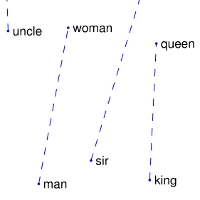
\includegraphics[width=\linewidth]{images/glove_mw}
\end{minipage}
\begin{minipage}{.3\textwidth}
  \centering
  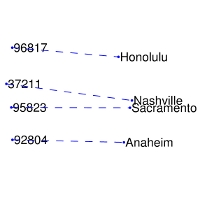
\includegraphics[width=\linewidth]{images/glove_cz}
\end{minipage}
\begin{minipage}{.3\textwidth}
  \centering
  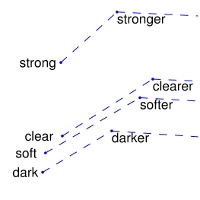
\includegraphics[width=\linewidth]{images/glove_cs}
\end{minipage}
\caption{Word embeddings give insightful correlations between similar and different words. For example, we can obtain several relations between female and male people, between zip codes and cities or between comparatives and superlatives \cite{pennington2014glove}.}
\label{fig:glove}
\end{figure}

\paragraph{Bag of Contexts.} In addition, CMU's Machine Learning Department provides another way to compare words. Their Never-Ending Language Learner provides information in which contexts certain words are used online \cite{nell_pairs}. We can create a corpus containing all different contexts. Similar to the bag-of-words approach, we can then count the occurrences of the words in the corpus' contexts. However, the resulting data is very sparse and Euclidean distance will not work well to compare the ``bag-of-contexts'' representations, i.e. other measurements such as the cosine distance are preferred.

\subsection{Image Features}
\label{sec:imagefeatures}

Similarly, there also exist ways to extract useful features from image data. In particular, this work focuses on neutral networks that learn to represent images in a way that images of different classes can be seperated well where images of the same class might share similar features.\\

\paragraph{CNN Features.} As a primary example, we use Convolutional Neural Network (CNN) architectures that learn to represent images with convolutional, pooling and activation layers and later map the representations to target classes with fully-connected layers. In this way, we can cut off the fully-connected layers to extract lower-dimensional feature representations for the input image data. Figure \ref{fig:cnnfeatures} visualizes such features learned on the ImageNet dataset \cite{krizhevsky2012imagenet}.

\begin{figure}[h]
    \centering
    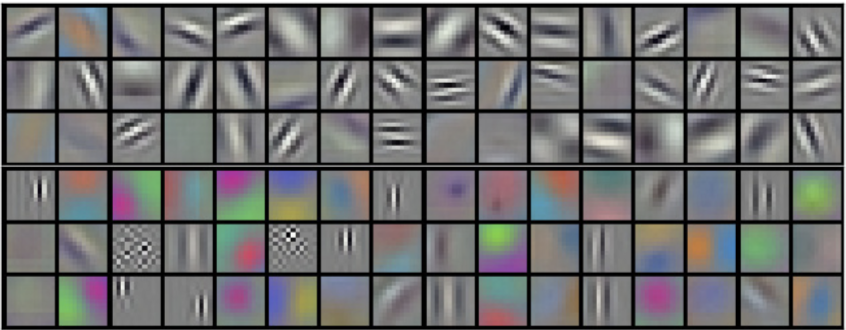
\includegraphics[width=0.8\textwidth]{images/cnn_features}
    \caption{Convolutional Neural Networks learn to represent images in lower-dimensional feature maps by applying convolutions to the image and averaging local neighborhoods (pooling) \cite{krizhevsky2012imagenet}.}
    \label{fig:cnnfeatures}
\end{figure}